\documentclass[11pt]{article}
\usepackage[a4paper, left=1.4cm, top=2.3cm, text={18.3cm, 25.2cm}]{geometry}
\usepackage[T1]{fontenc}
\usepackage[utf8]{inputenc}
\usepackage[slovak]{babel}
\usepackage{hyperref}
\usepackage{lmodern}
\usepackage{graphicx} % Required for inserting images

\title{IVH projekt - Dokumentácia
        }
\author{Jaroslav Mervart}
\date{May 2024}

\begin{document}

\maketitle

\section{Blokový návrh}
\begin{figure}[h]
    \centering
    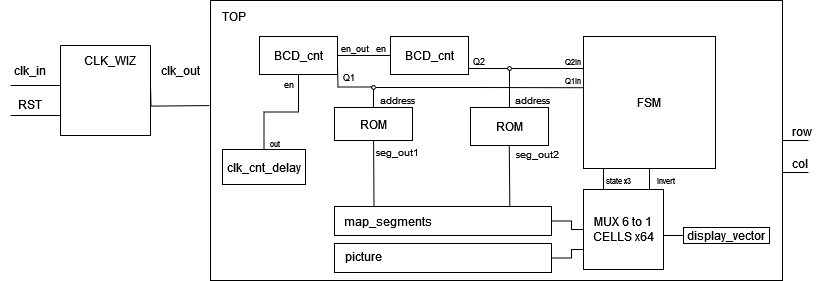
\includegraphics[width=0.60\linewidth]{rtl.drawio.png}
    \caption{RTL schéma}
    \label{fig:rtl}
\end{figure}

\section{Konštanty}
Konštanty použité s dvoma hodinovými čítačmi boli nasledujúce:

\begin{enumerate}
    \item \verb|constant maxcnt : integer := 50_000 - 1;| 
    \item \verb|constant delay : integer := 25_000_000 - 1;|
\end{enumerate}
Prvá konštanta definuje rýchlosť, akou striedame riadky, čo je každých $50\_000$ taktov, teda každé 2ms.
\begin{equation}
    25Mhz * 0.002
\end{equation}
Druhá konštanta je zodpovedná za inkrementovanie BCD čítača po každej sekunde, teda každých $25 mil.$ taktov. 
\section{FSM}
\begin{figure}[h]
    \centering
    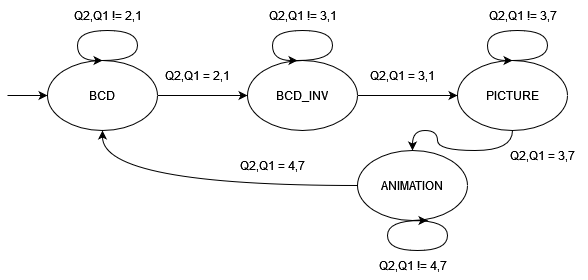
\includegraphics[width=0.45\linewidth]{fsm_diagram.png}
   \caption{  \centering Počiatočný stav je BCD zobrazenie }
    \label{fig:fsm_dia}
\end{figure}
\newpage
\newpage
%-----------------------------------------------------------------------------------------------------------

\section{Simulácie}
Projekt obsahuje 3 simulácie pre komponenty ROM, TOP a FSM. Okrem simulácie pre TOP sú zvyšné dve simulácie schopné otestovať dané komponenty pomocou konštrukcií \verb|assert|.
\subsection{Simulácia komponenty ROM}
\begin{figure}[h]
    \centering
    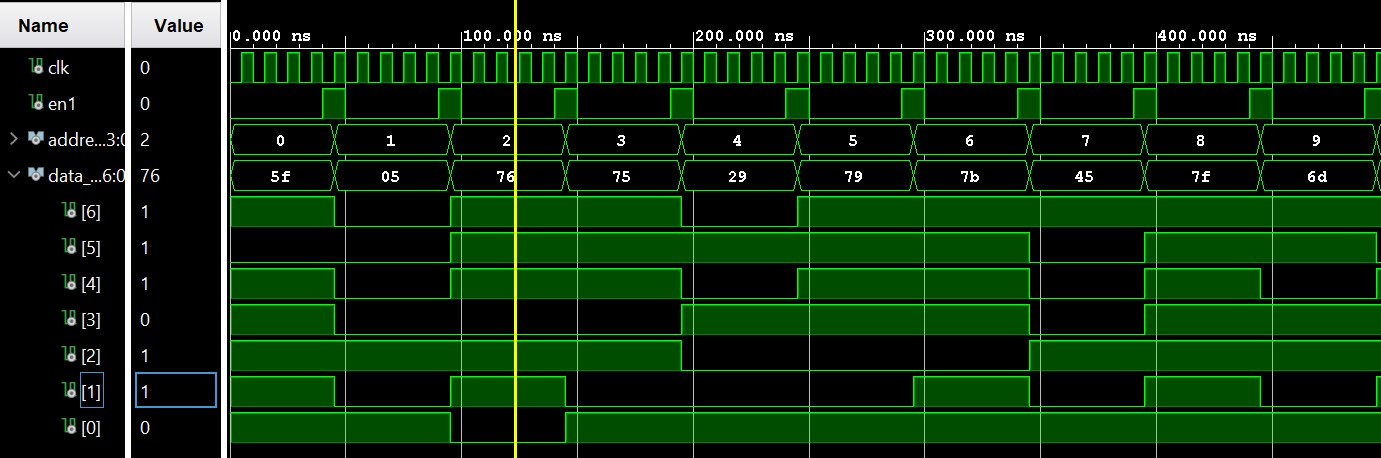
\includegraphics[width=0.6\linewidth]{ROM_sim.jpg}
   \caption{  \centering Pri hodnote BCD čítača $2$ kontrolujeme, či je výstup správny, teda či sa dáta zhodujú so segmentami potrebnými pre rozsvietenie čísla $2$.  }
    \label{fig:rom}
\end{figure}
\subsection{Simulácia komponenty FSM}
\begin{figure}[h]
    \centering
    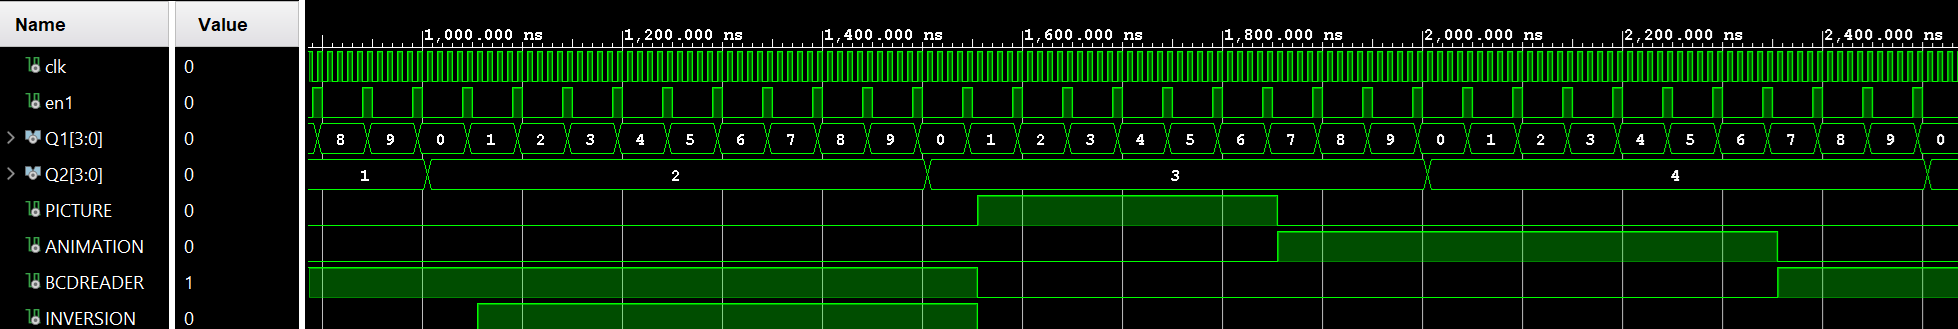
\includegraphics[width=1\linewidth]{FSM_tb.png}
   \caption{  \centering Kontroluje sa napríklad zapnutie inverzie pri hodnote BCD $21$, ale aj hodnoty stavov pri BCD hodnotách $35$ (Obrázok), $37$ (Animácia) a $47$ (Zobrazenie BCD).  }
    \label{fig:FSM}
\end{figure}
\subsection{Simulácia komponenty TOP }
\begin{figure}[h]
    \centering
    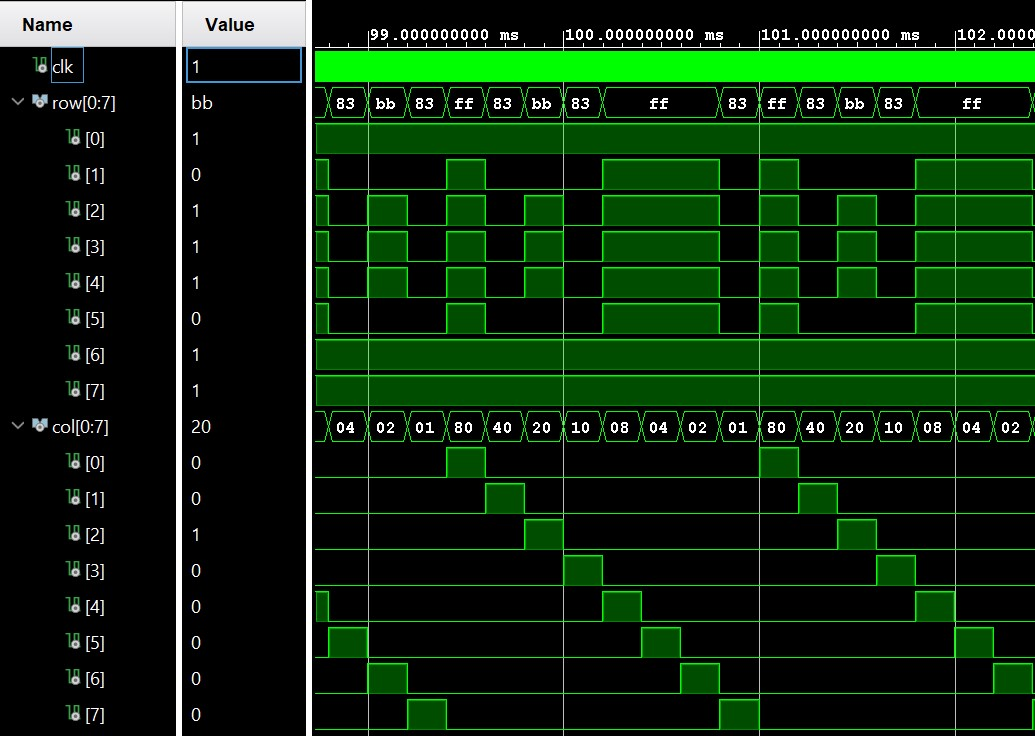
\includegraphics[width=0.5\linewidth]{top_sim.jpg}
   \caption{  \centering Simulácia top entity má hodinový signál nastavený na $2$ns, čo znamená že keď napríklad pozorujeme zmenu čísla na $100$ms, tak v skutočnosti to trvá $1$s  }
    \label{fig:top}
\end{figure}
\newpage
%-----------------------------------------------------------------------------------------------------------

\section{Dodatok}
V entite TOP sa nachádza $2*13$ procesov mapujúcich segmenty na bunky. Pre ujasnenie tohto rozhodnutia som priložil ústrižok z mojích poznámok tvorených súčasne s projektom.
\begin{figure}[h]
    \centering
    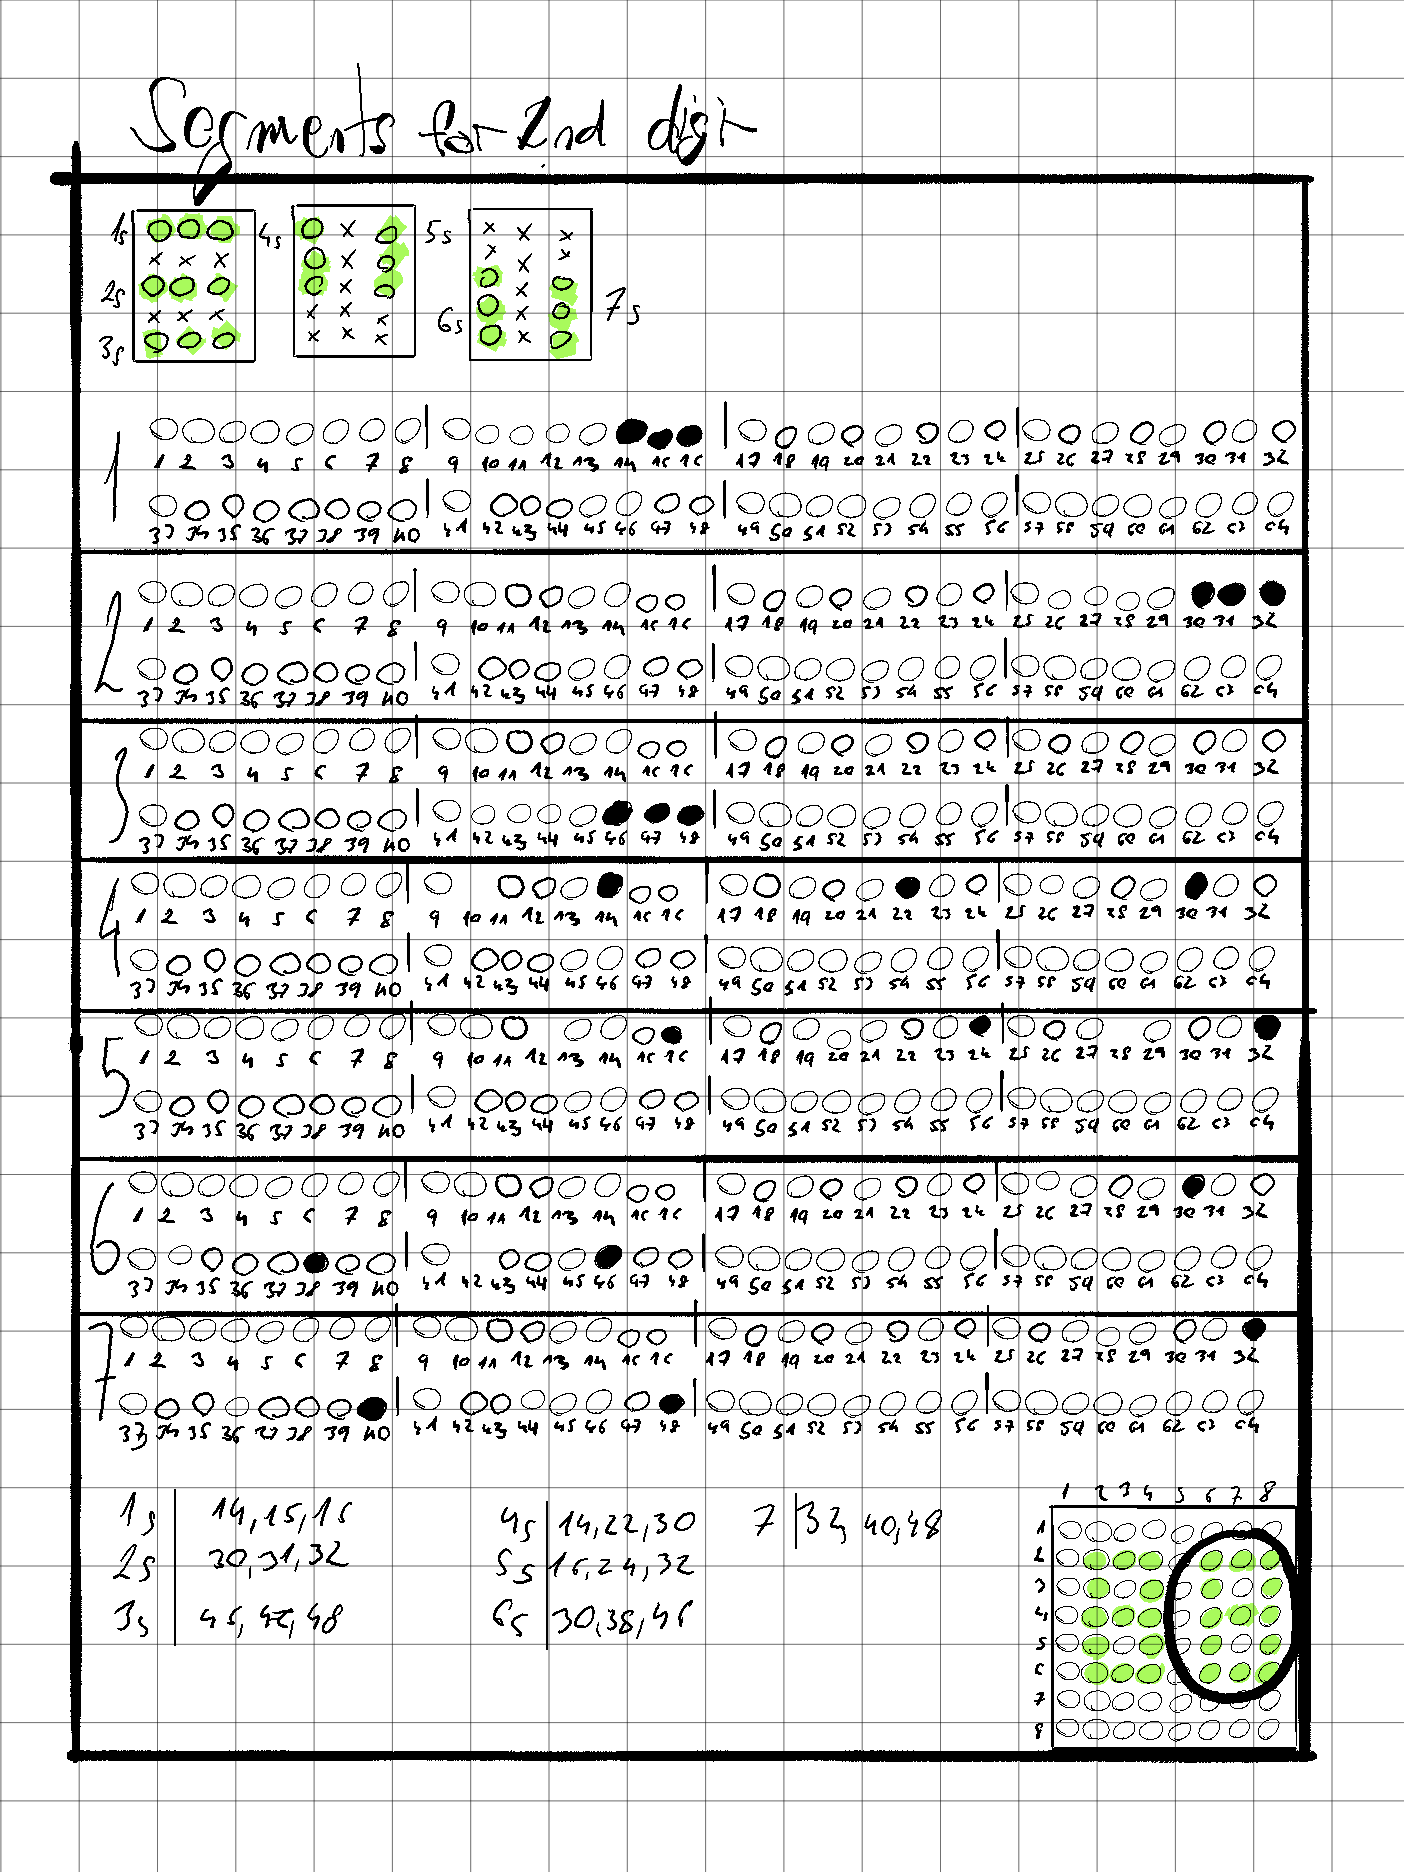
\includegraphics[width=0.75\linewidth]{IVH - page 4.png}
    \caption{Tento spôsob bol použitý na mapovanie buniek do segmentov}
    \label{fig:segment_mapping}
\end{figure}
\section{Odkaz na video}
\href{https://youtu.be/sGCAi2_AysI}{https://youtu.be/sGCAi2_AysI}
\end{document}
